\chapter{Introduction}
\label{chapter:intro}
\section{Why Anomalies Matter?}
As the elderly population increases, demand for outpatient services rises, which increases the operation cost in hospital~\cite{gupta2008appointment}\cite{hulshof2012taxonomic}. This phenomenon requires improvements on the efficiency in healthcare service institutes. Among several potential aspects of improving efficiency, one expectation is to make the whole visit more smoothly. 

A patient visit to the hospital consists of several phases. From enrolling to doctor treatment, each phase are affected by many factors which could result in an unpleasant experience. Examples are long waiting time, disordered treatment procedures etc. Studying unexpected care-flows is an important method to help provide better visit experience. From studying these abnormal cases, administrative stuffs can understand the reasons for causing the problems. Thus, the stuffs can balance resources allocated in the hospital for smoother service in the future. What is better, if real-time anomaly detection is available, then the hospital can provide necessary help to the patient in time. This thesis aims at developing practical anomaly detection methods on patient visits data.

\section{Background: State Flow of the X-Akseli System}
Studies in this thesis are based on data extracted from Oulu University Hospital, generated by X-Akseli queue system which aims at making patient reception fluent and effortless. This section describes how the X-Akseli reservation system works, in order to give the reader a general idea about how the data was produced. Patience privacy has been protected by using anonymous ids. The reservation system has gone through several updates while recording these data. Considering this situation, the discussion in this thesis adheres to the latest system, version 1.18.3.

Assuming a patient has already made a reservation online. A typical visit scenario to the hospital is as follow. The patient arrives at the hospital lobby. Then the patient takes a queue number at the self-service kiosk, with information showing in which area the patient should wait. Next, the patient goes to the correct waiting area, shows the queue number to another kiosk in the area to check in. After this, the patient can sit down and wait to be called by the doctor. When the doctor is available, the doctor will call the patient, treat the patient and close the whole visit. If assisted diagnose is needed, the doctor may pause the treatment. After other diagnoses are finished, the doctor then continues the treatment. In small departments, there may be no separation of waiting area and lobby. In this case, the first two steps will be integrated. The patient will not have to show the queue number to another kiosk. However, there will still be two events recorded in the back end system, but with zero transition time. The whole procedure is shown in Figure~\ref{fig:visit} and the state flow of the back end system is shown in Figure~\ref{fig:state}

\begin{figure}
	\begin{center}
		\includegraphics[width=0.8\textwidth]{images/visit}
		\caption{A typical visit scenario in hospital.}
		\label{fig:visit}
	\end{center}
\end{figure}

\begin{table}
	\caption{One example visit to the hospital.}
	\label{table:example}
	\begin{tabular}{|c|c|c|}
		\hline
		 reservationid &      eventname      &          time	\\ \hline

	      21332189 & ENROLLING           & 2014-03-26 08:02:42.353	\\ \hline
	      21332189 & ARRIVED\_IN\_HOSPITAL & 2014-03-26 08:02:42.517	\\ \hline
    	  21332189 & WAITING             & 2014-03-26 08:03:29.007	\\ \hline
	      21332189 & CALLED              & 2014-03-26 08:07:15.061	\\ \hline
    	  21332189 & IN\_TREATMENT\_ROOM   & 2014-03-26 08:07:15.072	\\ \hline
	      21332189 & CLOSED              & 2014-03-26 08:13:11.002	\\ \hline
	\end{tabular}
\end{table}

\begin{sidewaysfigure}
	\begin{center}
		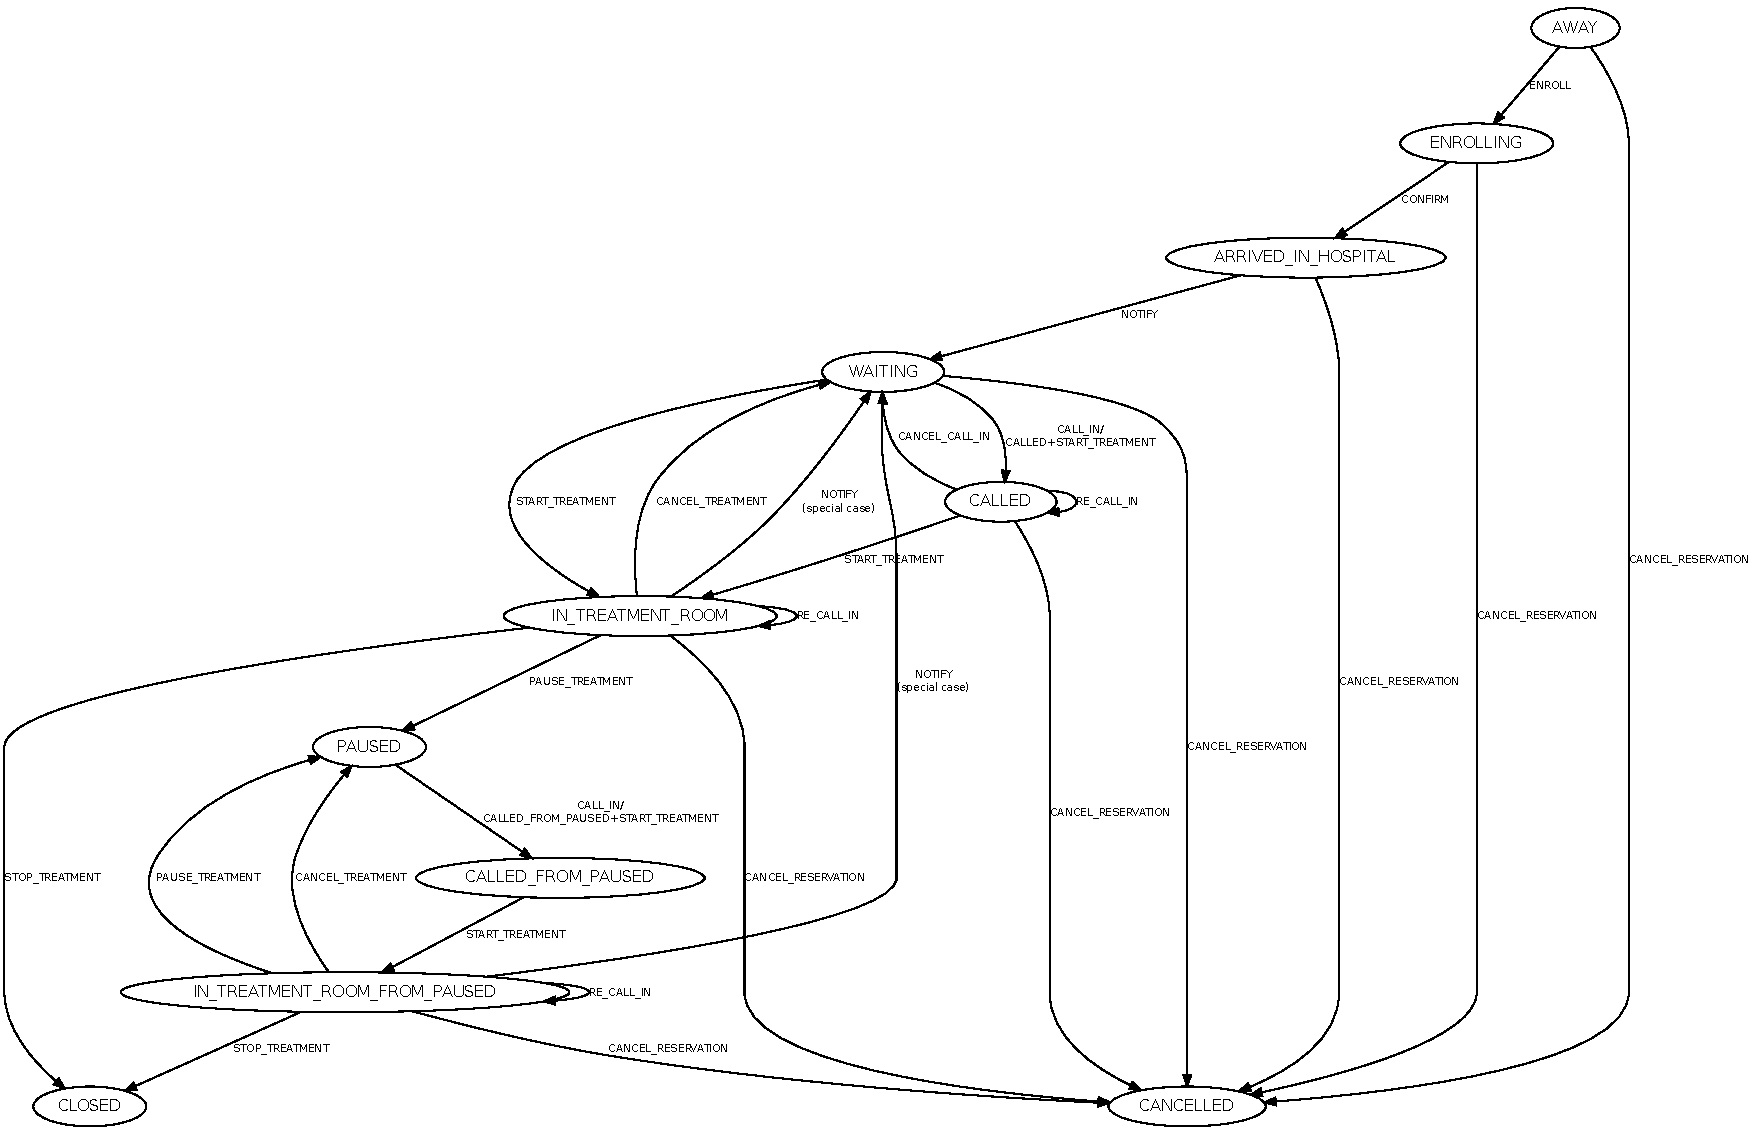
\includegraphics[width=0.8\textwidth]{images/patientFsm}
		\caption{State flow in X-Akseli system, version 1.18.3.}
		\label{fig:state}
	\end{center}
\end{sidewaysfigure}

One example visit is listed in Table~\ref{table:example}. Notice that, there are 6 events in this visit. However, the first two events \texttt{ENROLLING} and  \texttt{ARRIVED\_IN\_HOSPITAL} happened in less than 1 second. This also happens to the 4th and 5th events, \texttt{CALLED} and \texttt{IN\_TREATMENT\_ROOM}. It can be considered that the two events in these two pairs happen simultaneously. To reduce redundant information, in this thesis, only following 7 events are considered. They are: \texttt{ENROLLING}, \texttt{WAITING}, \texttt{IN\_TREATMENT\_ROOM}, \texttt{PAUSED}, \texttt{IN\_TREATMENT\_ROOM\_FROM\_PAUSED}, \\ \texttt{CLOSED}, and \texttt{CANCELLED}.

\section{Problem Description}
Spotting an anomaly from hospital visits can be seen as finding outliers in a database containing time series entries. The assumption is that, the number of anomalies in the database is quite few compared to the number of normal entries. One naive approach to solve this problem is extreme value detection~\cite{aggarwal2013introduction}. The idea is to set a threshold and classify any entry which has a value exceeds the threshold to be an anomaly. In the patient visits case, the threshold can be set to be a specific waiting time. Any visits have a longer time than the threshold is an anomaly. However, this approach have some obvious drawbacks.Due to the hard assignment, performance of this method heavily depends on the selection of the threshold value. However, the boundary between anomaly and normal data is not clear. There could be a ``gray area'' around this threshold value. Additionally, definition of anomalies in patient visit is not only limited to durations. Anomalies may also consists of strange behaviours of the patient states, for example, being in \texttt{WAITING} states for several times. This may be caused by going to wrong waiting areas.

An alternative approach is to scoring each entry by showing how likely it could be an anomaly~\cite{gupta2014outlier}. Then, anomalies are detected based on these scores. Typical methods include clustering methods and Markovian models. This approach considers anomalies from overview aspect. The concept is that, a single minor misbehaviour doesn't necessarily lead to an anomaly. It is a sequence of uncommon behaviours that results in anomalies. This thesis decides to explore the problem using this approach.

\section{Thesis Structure}
The thesis aims at suggesting a practical method for detecting anomalies in hospital visits. The structure of this thesis is organized as follow. Chapter~\ref{chapter:clustering} introduces potential clustering method. Chapter~\ref{chapter:generative} introduces potential generative model methods. Then Chapter~\ref{chapter:Experiment} first describes more details and pre-process executed on the data used in the experiment. Then this chapter compares strength and drawbacks of these methods, discusses their applicability, and describes the experiment setup. Finally, Chapter~\ref{chapter:results} presents and analyses the obtained results.